% Native editable composition from verified, unchanged IDE images.
\begin{figure}[htbp]
\centering
\sbox0{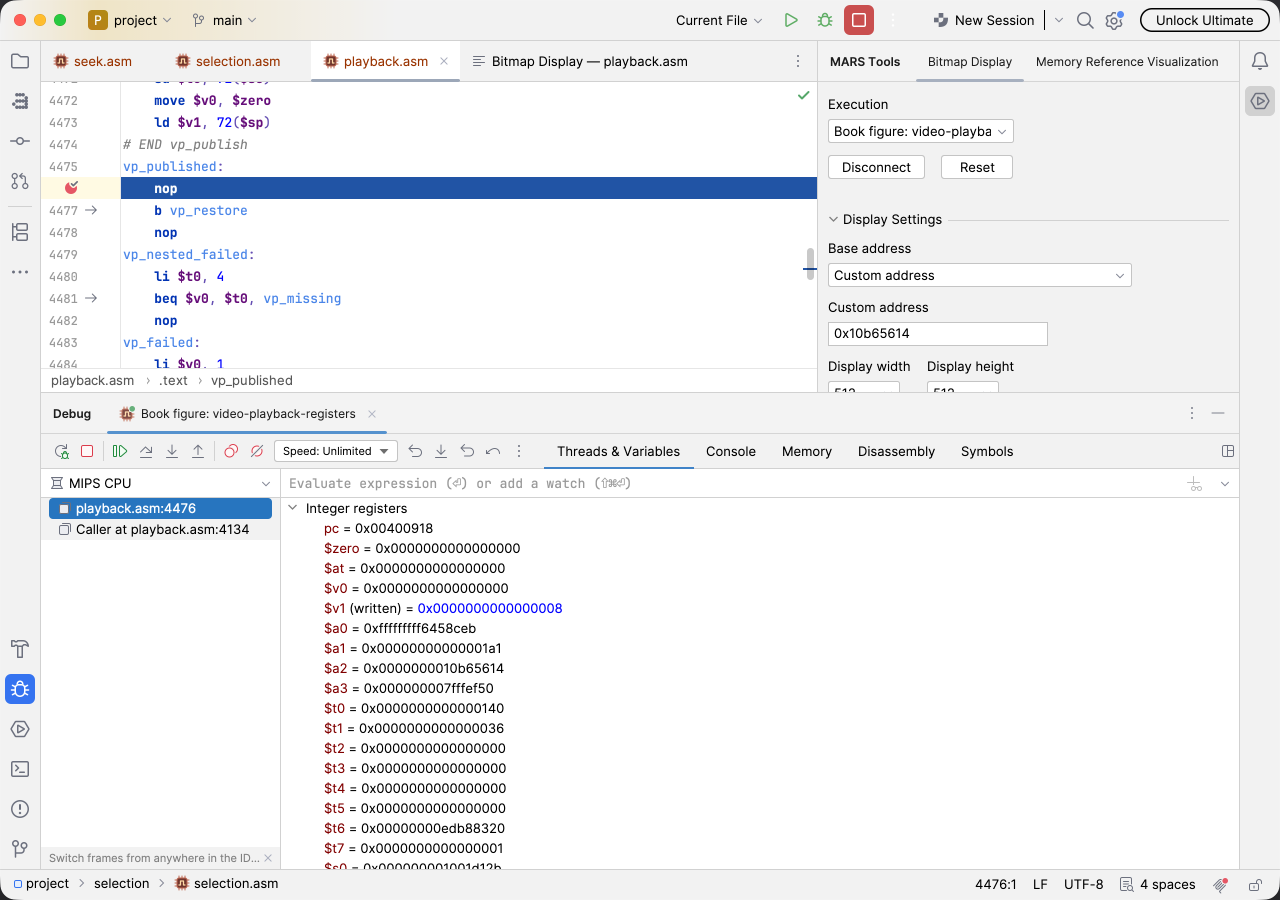
\includegraphics[artifact]{packages/034-lossless-video/captures/video-playback-progress/registers.png}}
\sbox2{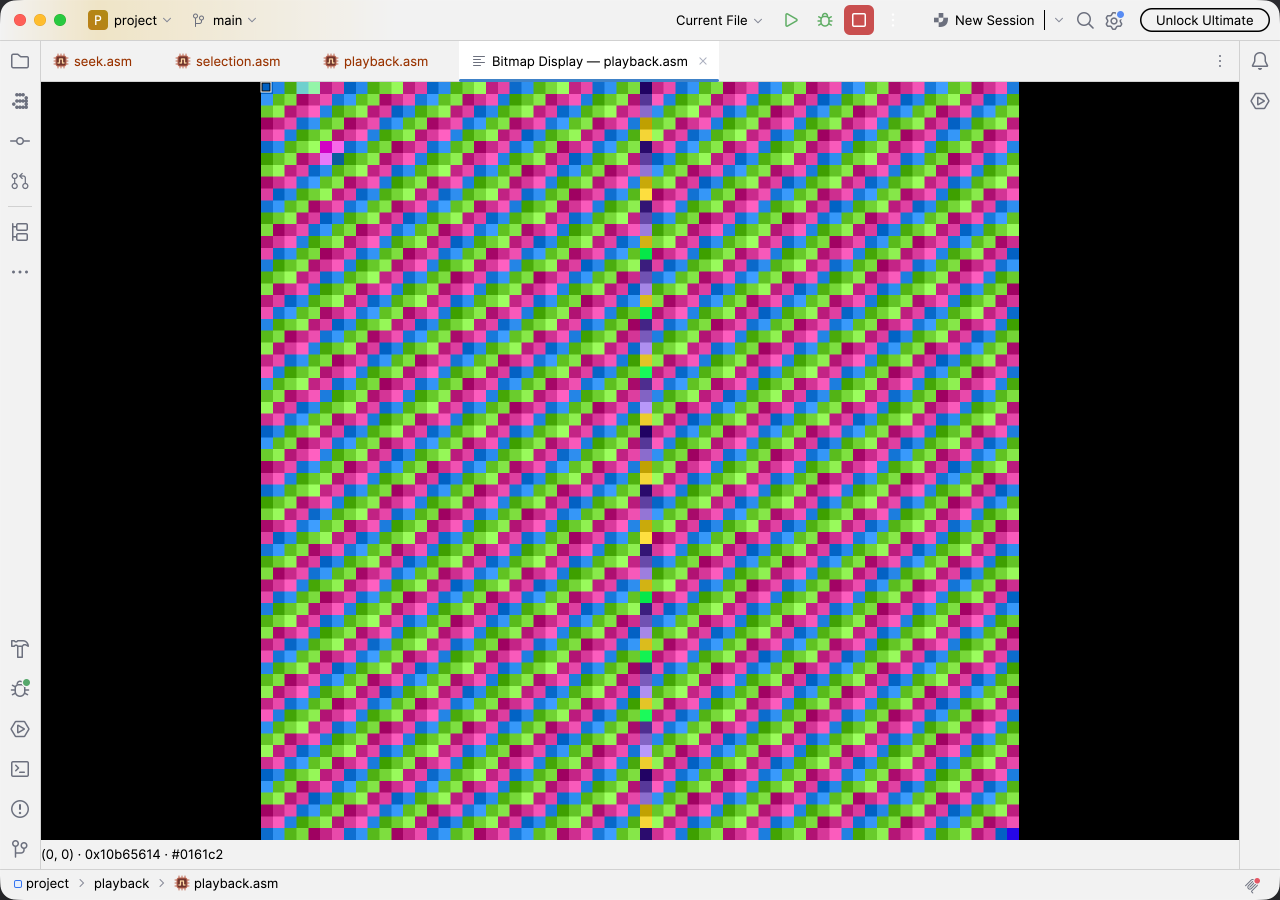
\includegraphics[artifact]{packages/034-lossless-video/captures/video-playback-progress/bitmap.png}}
\sbox4{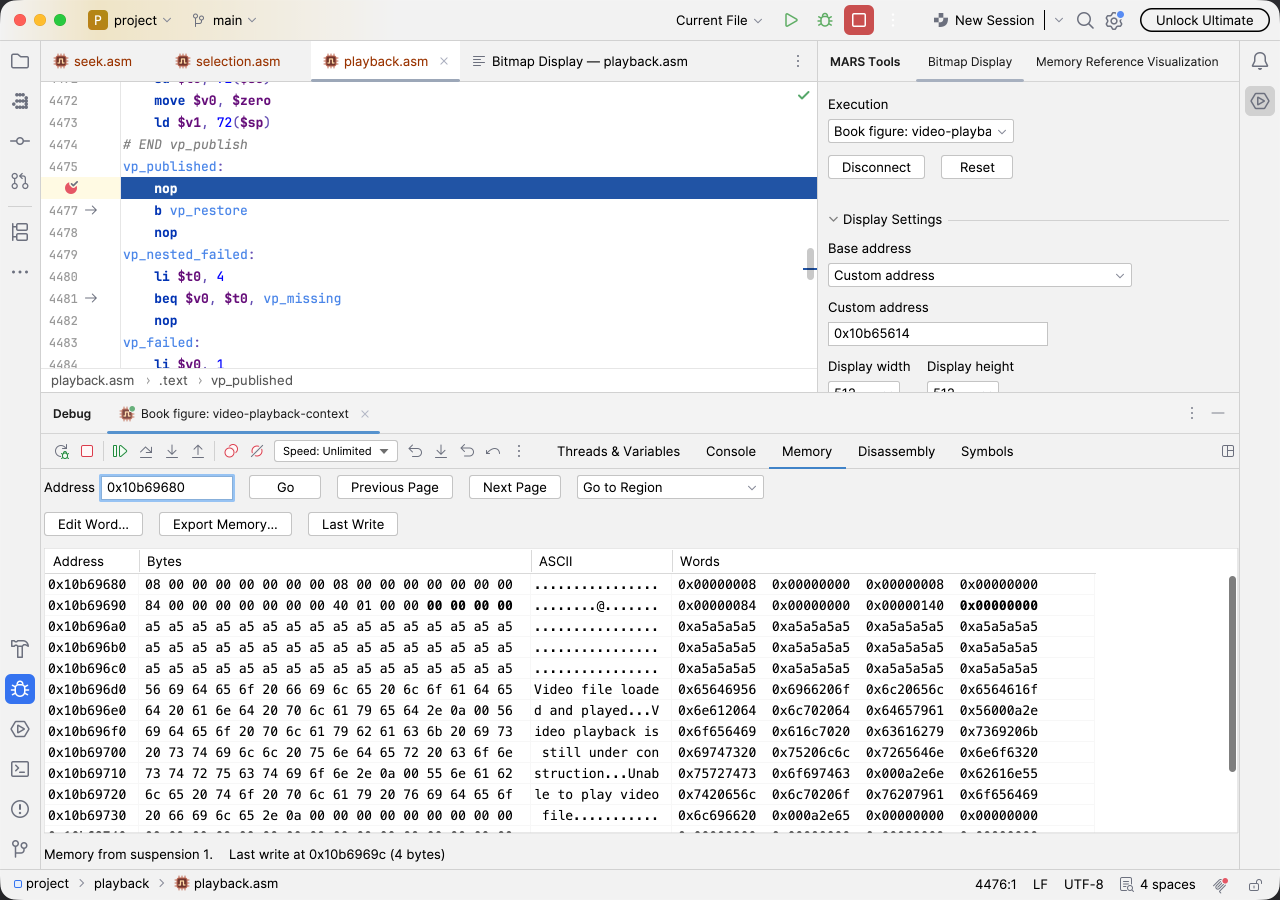
\includegraphics[artifact]{packages/034-lossless-video/captures/video-playback-progress/context.png}}
\edef\MARSplaybacksourceLeft{\the\dimexpr0.036718750\wd0\relax}
\edef\MARSplaybacksourceBottom{\the\dimexpr0.774444444\ht0\relax}
\edef\MARSplaybacksourceRight{\the\dimexpr0.611718750\wd0\relax}
\edef\MARSplaybacksourceTop{\the\dimexpr0.170000000\ht0\relax}
\edef\MARSplaybackbitmapLeft{\the\dimexpr0.199218750\wd2\relax}
\edef\MARSplaybackbitmapBottom{\the\dimexpr0.060000000\ht2\relax}
\edef\MARSplaybackbitmapRight{\the\dimexpr0.199218750\wd2\relax}
\edef\MARSplaybackbitmapTop{\the\dimexpr0.084444444\ht2\relax}
\edef\MARSplaybackcontextLeft{\the\dimexpr0.520312500\wd4\relax}
\edef\MARSplaybackcontextBottom{\the\dimexpr0.312222222\ht4\relax}
\edef\MARSplaybackcontextRight{\the\dimexpr0.139843750\wd4\relax}
\edef\MARSplaybackcontextTop{\the\dimexpr0.634444444\ht4\relax}
\edef\MARSplaybackreturnsLeft{\the\dimexpr0.246093750\wd0\relax}
\edef\MARSplaybackreturnsBottom{\the\dimexpr0.310000000\ht0\relax}
\edef\MARSplaybackreturnsRight{\the\dimexpr0.554687500\wd0\relax}
\edef\MARSplaybackreturnsTop{\the\dimexpr0.638888889\ht0\relax}
\begin{tikzpicture}[alt={Four annotated IDE details at vp_published. Detail 1 marks the next instruction after final publication. Detail 2 shows the last accepted 64 by 64 picture. Detail 3 shows little-endian low/high word pairs: eight accepted pictures, 8 late intervals, maximum lateness 132 milliseconds, and scheduled logical duration 320 milliseconds. These are actual host-clock observations, not the scripted zero-lateness example. Detail 4 shows success v0 equal to zero and v1 equal to eight accepted pictures.}]
\node[anchor=north west,inner sep=0,font=\small\bfseries] (source-title) at (6mm,0) {Paused final publication};
\node[anchor=north west,inner sep=0] (source) at ([yshift=-1mm]source-title.south west) {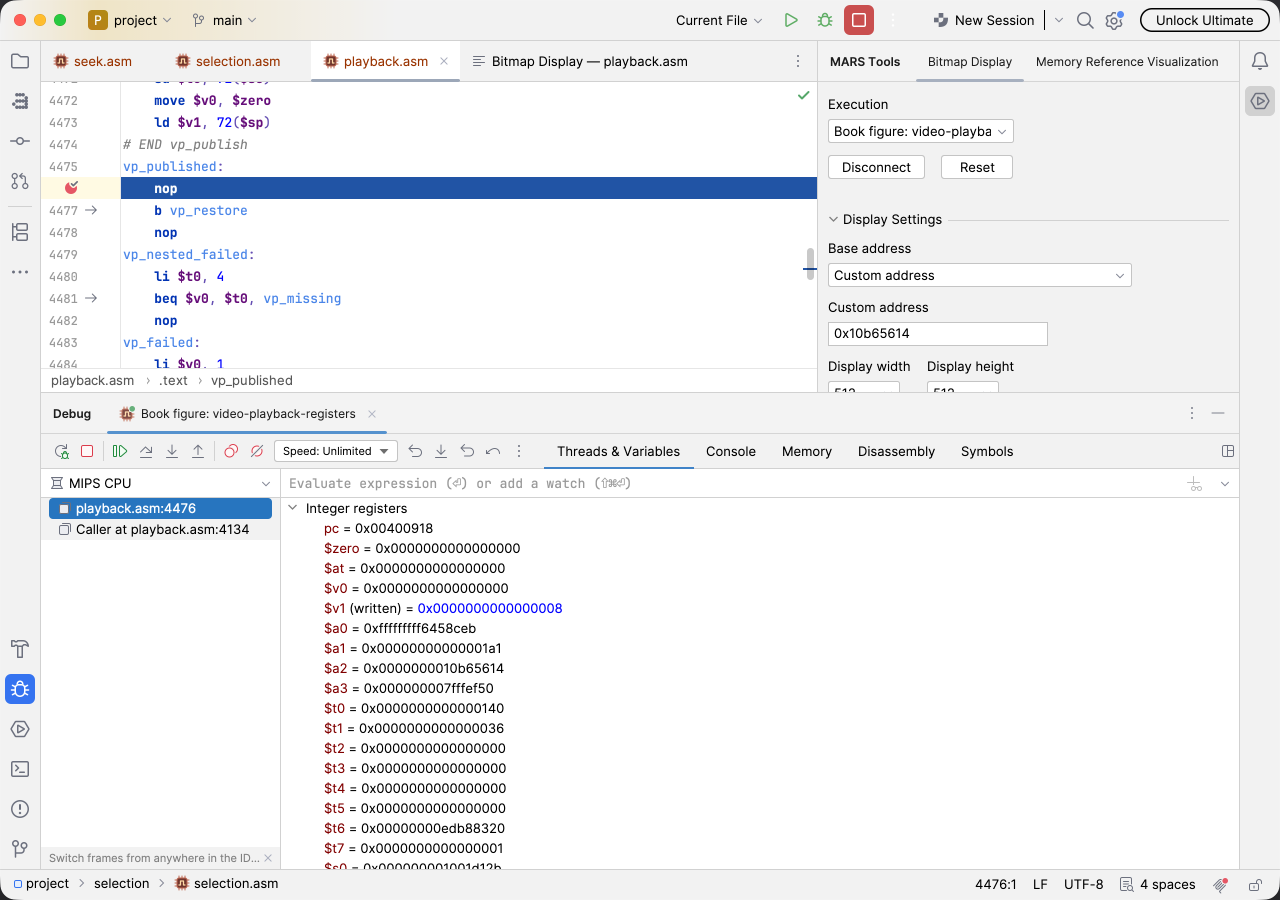
\includegraphics[width=0.66\linewidth,artifact,trim={\MARSplaybacksourceLeft{} \MARSplaybacksourceBottom{} \MARSplaybacksourceRight{} \MARSplaybacksourceTop{}},clip]{packages/034-lossless-video/captures/video-playback-progress/registers.png}};
\begin{scope}[shift={(source.south west)},x={($(source.south east)-(source.south west)$)},y={($(source.north west)-(source.south west)$)}]
\draw[black,line width=0.7pt] (0.168888889,0.080000000) rectangle (0.288888889,0.520000000);
\node[draw=black,fill=white,circle,inner sep=1.5pt,font=\footnotesize] at ($(0.168888889,0.520000000)+(-3mm,0)$) {1};
\end{scope}
\node[anchor=north west,inner sep=0,font=\small\bfseries] (bitmap-title) at ([yshift=-3mm]source.south west) {Last accepted picture};
\node[anchor=north west,inner sep=0] (bitmap) at ([yshift=-1mm]bitmap-title.south west) {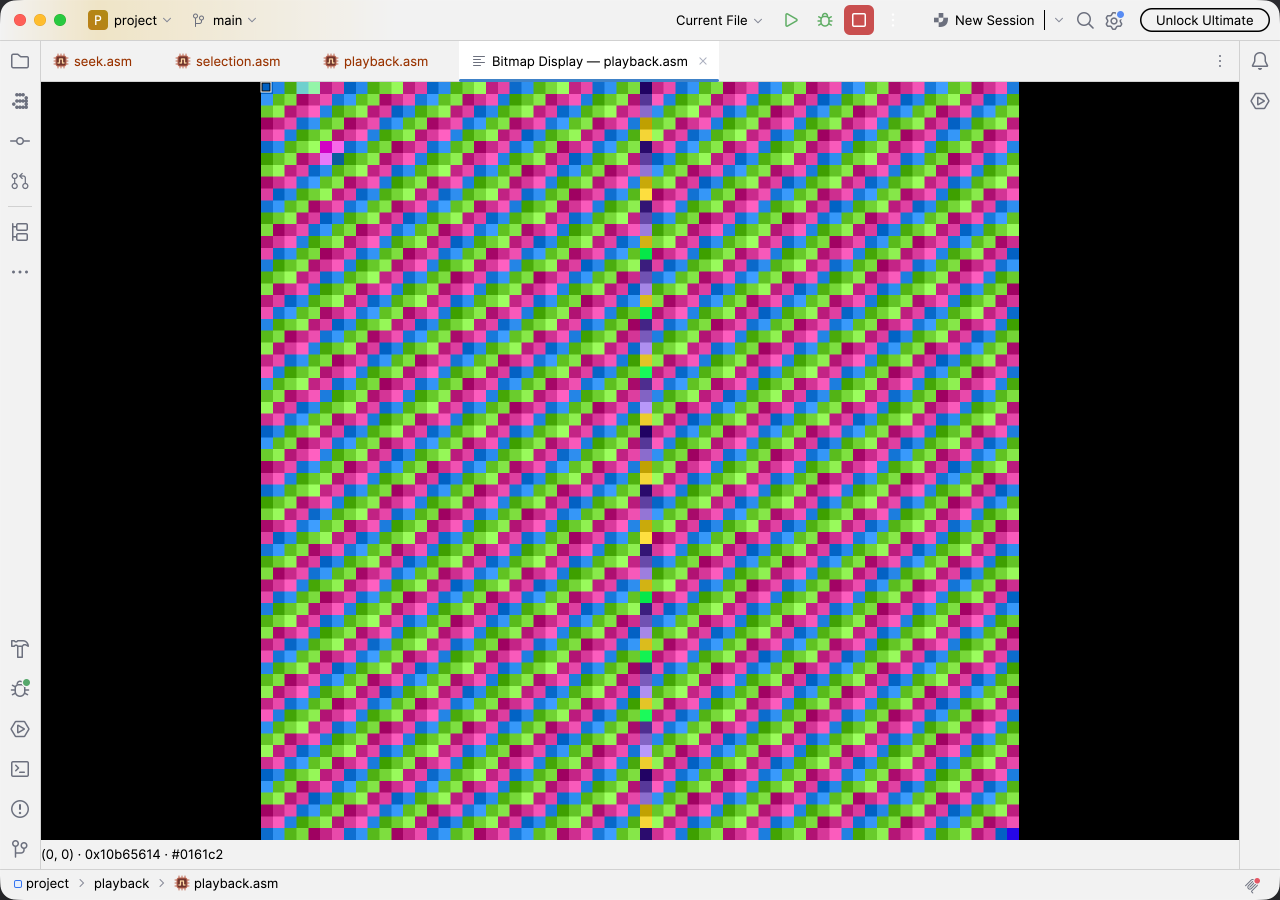
\includegraphics[width=0.5\linewidth,artifact,trim={\MARSplaybackbitmapLeft{} \MARSplaybackbitmapBottom{} \MARSplaybackbitmapRight{} \MARSplaybackbitmapTop{}},clip]{packages/034-lossless-video/captures/video-playback-progress/bitmap.png}};
\begin{scope}[shift={(bitmap.south west)},x={($(bitmap.south east)-(bitmap.south west)$)},y={($(bitmap.north west)-(bitmap.south west)$)}]
\draw[black,line width=0.7pt] (0.007792208,0.007792208) rectangle (0.992207792,0.992207792);
\node[draw=black,fill=white,circle,inner sep=1.5pt,font=\footnotesize] at ($(0.007792208,0.992207792)+(-3mm,0)$) {2};
\end{scope}
\node[anchor=north west,inner sep=0,font=\small\bfseries] (context-title) at ([yshift=-3mm]bitmap.south west) {Observed progress and real-clock lateness};
\node[anchor=north west,inner sep=0] (context) at ([yshift=-1mm]context-title.south west) {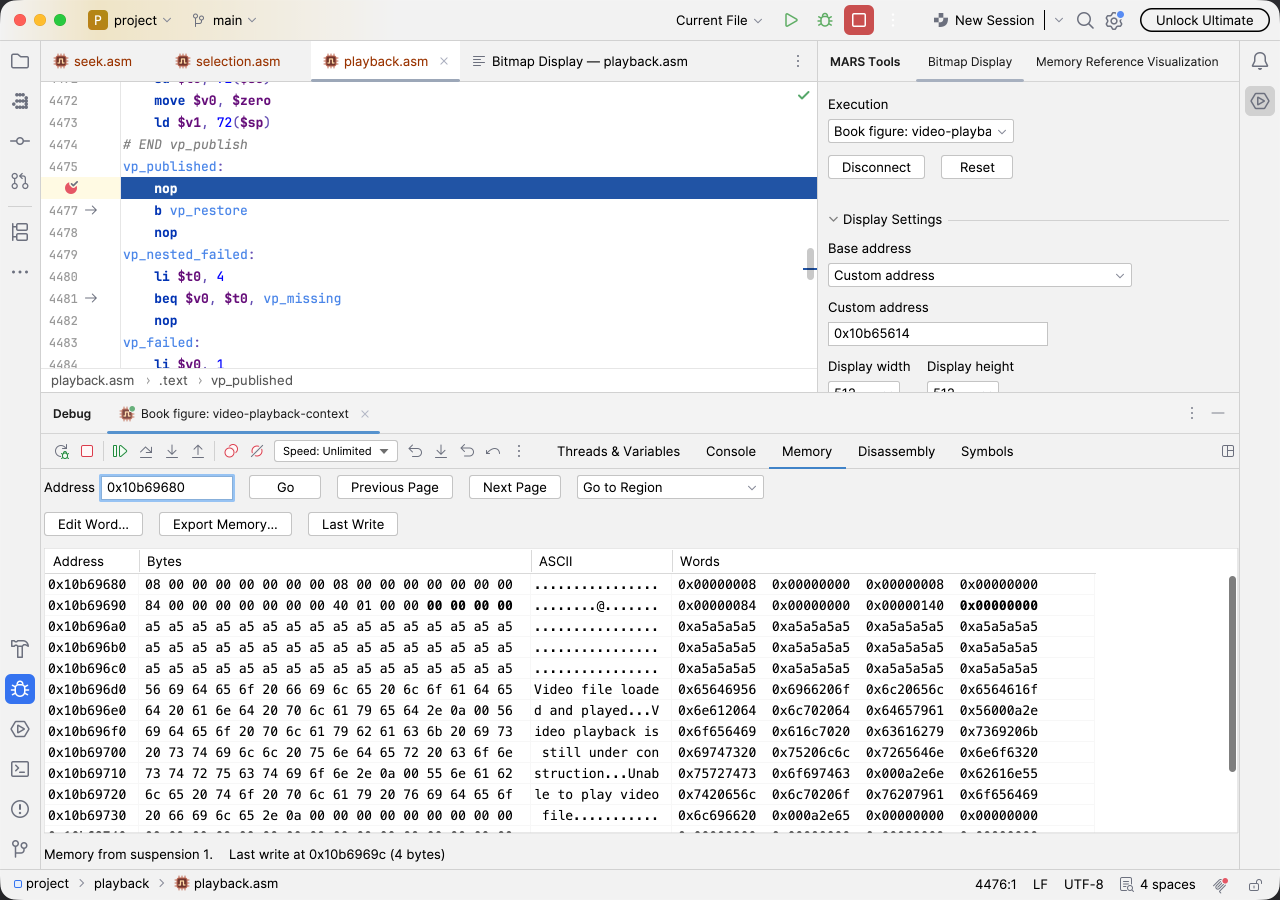
\includegraphics[width=0.74\linewidth,artifact,trim={\MARSplaybackcontextLeft{} \MARSplaybackcontextBottom{} \MARSplaybackcontextRight{} \MARSplaybackcontextTop{}},clip]{packages/034-lossless-video/captures/video-playback-progress/context.png}};
\begin{scope}[shift={(context.south west)},x={($(context.south east)-(context.south west)$)},y={($(context.north west)-(context.south west)$)}]
\draw[black,line width=0.7pt] (0.013793103,0.062500000) rectangle (0.986206897,0.937500000);
\node[draw=black,fill=white,circle,inner sep=1.5pt,font=\footnotesize] at ($(0.013793103,0.937500000)+(-3mm,0)$) {3};
\end{scope}
\node[anchor=north west,inner sep=0,font=\small\bfseries] (returns-title) at ([yshift=-3mm]context.south west) {Success and accepted picture count};
\node[anchor=north west,inner sep=0] (returns) at ([yshift=-1mm]returns-title.south west) {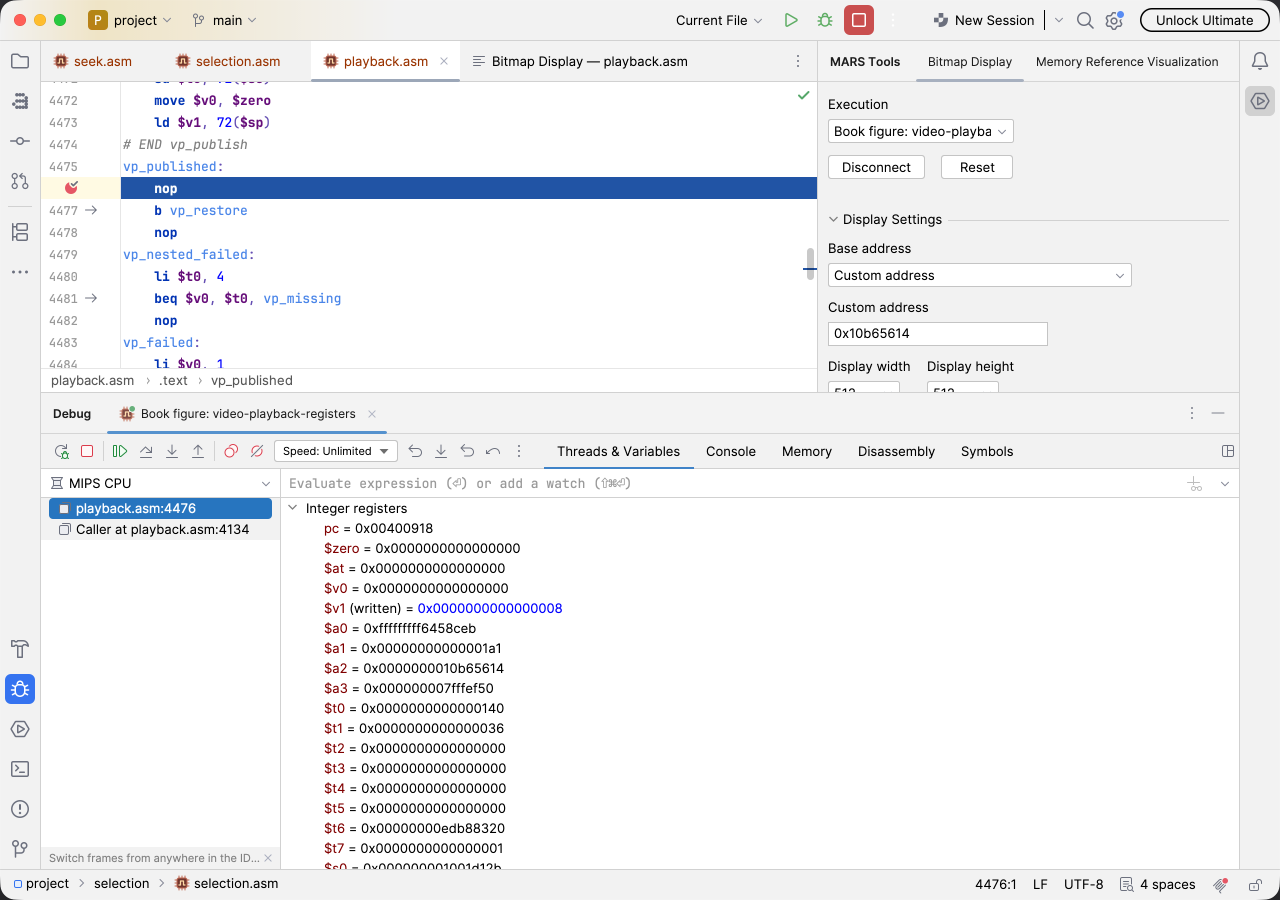
\includegraphics[width=0.5\linewidth,artifact,trim={\MARSplaybackreturnsLeft{} \MARSplaybackreturnsBottom{} \MARSplaybackreturnsRight{} \MARSplaybackreturnsTop{}},clip]{packages/034-lossless-video/captures/video-playback-progress/registers.png}};
\begin{scope}[shift={(returns.south west)},x={($(returns.south east)-(returns.south west)$)},y={($(returns.north west)-(returns.south west)$)}]
\draw[black,line width=0.7pt] (0.023529412,0.065217391) rectangle (0.976470588,0.934782609);
\node[draw=black,fill=white,circle,inner sep=1.5pt,font=\footnotesize] at ($(0.023529412,0.934782609)+(-3mm,0)$) {4};
\end{scope}
\end{tikzpicture}
\par\smallskip
\begin{minipage}{\linewidth}
\small
\begin{enumerate}
\item The completed result has been published before the checkpoint \texttt{nop}.
\item The picture is frame seven. This fixture ends with an unchanged record, so its pixels match frame six; the picture alone cannot establish the accepted count.
\item Low/high pairs show eight accepted pictures, 8 late intervals, maximum lateness 132\,ms and scheduled duration \texttt{0x140} = 320\,ms. Another real-clock launch may report different lateness.
\item \texttt{\$v0} is zero; \texttt{\$v1} is eight pictures. This return count is not an image byte count.
\end{enumerate}
\end{minipage}
\caption{Completed playback with the real IDE clock. Three Debug launches reach the same checkpoint; the lateness values belong to the context view.}
\label{fig:video-playback-progress}
\end{figure}
